\documentclass[10pt,a4paper,twocolumn]{article}
\usepackage[left=1.5cm,right=1.2cm,top=1.3cm,bottom=2.0cm,columnsep=0.635cm,footskip=0.9cm]{geometry}
\usepackage[T1]{fontenc}
\usepackage{mathptmx}
\usepackage[scaled=.92]{helvet}
\usepackage{microtype}
\usepackage{ragged2e}
\usepackage{amsmath,amssymb,bm}
\usepackage{graphicx,xcolor}
\usepackage{booktabs,multirow,adjustbox}
\usepackage[group-separator={,}]{siunitx}
\usepackage{enumitem}
\usepackage{titlesec}
\usepackage{fancyhdr}
\usepackage[labelsep=period,justification=justified,singlelinecheck=on,font=footnotesize]{caption}
\captionsetup[figure]{name={Fig.}}
\usepackage[numbers,sort&compress]{natbib}\bibpunct{[}{]}{,}{n}{}{,}
\usepackage[hidelinks]{hyperref}
\input{gen/results_macros.tex}
\setlength{\parindent}{1.0em}\setlength{\parskip}{0pt}
\setlist{nosep,leftmargin=1.4em,itemsep=1pt}
\titleformat{\section}{\normalsize\bfseries}{\thesection.}{0.5em}{}
\titleformat{\subsection}{\normalsize\itshape}{\thesubsection.}{0.5em}{}
\titlespacing*{\section}{0pt}{9pt}{4pt}\titlespacing*{\subsection}{0pt}{6pt}{3pt}
\setlength{\textfloatsep}{8pt plus 2pt minus 2pt}\setlength{\floatsep}{7pt plus 2pt minus 2pt}\setlength{\intextsep}{7pt plus 2pt minus 2pt}
\setlength{\abovedisplayskip}{5pt plus 1pt minus 1pt}\setlength{\belowdisplayskip}{5pt plus 1pt minus 1pt}
\renewcommand{\arraystretch}{1.05}
\pagestyle{empty}
\fancypagestyle{firstpage}{\fancyhf{}\renewcommand{\headrulewidth}{0pt}\fancyfoot[C]{\fontsize{7}{8}\selectfont 2213-8463 \copyright\ 2027 The Authors. Published by Elsevier B.V. This is an open access article under the CC BY-NC-ND license (https://creativecommons.org/licenses/by-nc-nd/4.0)\\Peer-review under responsibility of the scientific committee of the NAMRI|SME.}}
\newcommand{\vect}[1]{\bm{#1}}
\DeclareMathOperator*{\argmin}{arg\,min}
\begin{document}
\thispagestyle{firstpage}
\twocolumn[{%
\begin{center}
{\fontfamily{phv}\selectfont\footnotesize Available online at www.sciencedirect.com}\\[2pt]
{\fontsize{17}{19}\selectfont Manufacturing Letters}\\[1pt]
{\fontsize{7}{8}\selectfont Manufacturing Letters 00 (2027) 000--000}\\[7pt]
{\fontsize{11}{13}\selectfont 55th SME North American Manufacturing Research Conference (NAMRC 55 2027)}\\[8pt]
{\fontsize{14}{17}\selectfont PARD: A plan-referenced framework for quantifying process execution deviations in fused filament fabrication}\\[7pt]
{\fontsize{11}{13}\selectfont [Author One]$^{\mathrm{a}}$, [Author Two]$^{\mathrm{b}}$, [Author Three]$^{\mathrm{a,}*}$}\\[3pt]
{\fontsize{7.5}{9}\selectfont\itshape $^{\mathrm{a}}$[First affiliation, Address, City and Postcode, Country]\\ $^{\mathrm{b}}$[Second affiliation, Address, City and Postcode, Country]}
\end{center}
\vspace{-2pt}{\fontsize{8}{9.5}\selectfont $^*$ Corresponding author. E-mail address: [author@institute.xxx]}\par
\vspace{3pt}\hrule\vspace{4pt}
\begin{minipage}{\textwidth}\fontsize{9}{11}\selectfont\justifying
\noindent\textbf{Abstract}\par\vspace{3pt}
Fused filament fabrication (FFF) builds parts from a prescribed plan of thermal, cooling, motion and extrusion conditions, but the conditions a printer reports executing may depart from that plan. Reconstructing the size and direction of these departures is difficult because the process variables differ in response dynamics and in how directly firmware telemetry observes them. This paper presents PARD, a plan-referenced framework that reconstructs multichannel execution deviations from built-in firmware telemetry. PARD combines explicit plan references, response-delay alignment, estimator selection by run-grouped cross-validation on development data, and a unified execution-fidelity score. It was developed on \printsDev{} nominal and single-excursion prints and evaluated on \printsTest{} mixed-excursion prints made with a LulzBot Mini 3 and PLA. Selection assigned delayed linear estimation to temperature, same-layer linear estimation to fan state, and learned estimation to speed and extrusion. On the mixed prints PARD reached an execution-fidelity AUC of \aucPard{} and an F1 score of \fonePard{}, compared with \aucBthree{} and \foneBthree{} for the strongest plan-aware learned baseline (paired $\Delta$AUC \dAucBthree{}, 95\% interval \dAucBthreeLo{} to \dAucBthreeHi{}). A one-layer thermal alignment reduced temperature-deviation error from \thDelayZero{} to \thDelayOne{}~\si{\celsius}. Interval coverage fell below its nominal target in three of four channels, and the evaluation includes an exploratory component. The results indicate the value of channel-adaptive reconstruction against a common plan reference for one printer, material and geometry.\par
\vspace{4pt}\noindent\copyright\ 2027 The Authors. Published by Elsevier B.V. This is an open access article under the CC BY-NC-ND license (https://creativecommons.org/licenses/by-nc-nd/4.0)\\
Peer-review under responsibility of the scientific committee of the NAMRI|SME.\par
\vspace{2pt}\noindent{\fontsize{8}{10}\selectfont\itshape Keywords: }{\fontsize{8}{10}\selectfont fused filament fabrication; process monitoring; plan referencing; firmware telemetry; execution fidelity; response delay}
\end{minipage}
\vspace{6pt}\hrule\vspace{8pt}
}]

\section{Introduction}
In fused filament fabrication (FFF), the G-code is the manufacturing plan. It prescribes the nozzle temperature, the part-cooling fan state, the feed rate and the extruded length that every layer should receive. The conditions that the machine executes can depart from this plan through operator or slicer overrides, firmware behaviour, actuator limits or deliberate manipulation. Whether a build followed its specified operating conditions, and by how much it departed from them, is a question of plan-execution fidelity. A quantitative answer supports process records, troubleshooting and the choice of build intervals that deserve closer inspection.

Several lines of work observe FFF processes against the plan. Corradini and Silvestri \cite{Corradini2022} built a digital twin that receives sensor data and the same G-code as the real machine, and provides process monitoring, condition monitoring and geometric accuracy control, including pausing a print on anomalies. Werkle et al.\ \cite{Werkle2024} compare the printed contour with the target contour obtained from G-code, layer by layer, using a camera. Fu and Li \cite{FuLi2025} predict process parameters from camera images with neural networks and add a corrective pause mechanism, without further sensors. Read et al.\ \cite{Read2024} use an instrumented extruder to fit a pressure map over flow rate and temperature, and use it to generate process parameters across machines and materials. A separate body of work detects sabotage of G-code or firmware from side channels such as power or multi-modal emissions \cite{Yu2020,Moore2017}, or from the G-code itself \cite{Ali2025}. These approaches establish capabilities for observation, quality monitoring and intervention. Quantitative reconstruction of the departures themselves, across heterogeneous firmware channels, is a distinct task that they do not address directly.

The task is hard because the channels cannot all be reconstructed by one observation model. Hotend temperature is a measured state with thermal response dynamics, so a commanded step is only partly visible in the layer in which it is issued. Fan telemetry can closely reflect the commanded state. Speed and extrusion involve command-to-execution relations that elementary layer-level ratios capture only partly. A learned model, finally, depends on the operating conditions represented in its training data, and a change in excursion direction or size between training and use can degrade it.

This paper proposes PARD, a plan-referenced execution-reconstruction framework. PARD forms a reference residual for each channel from the plan and the telemetry, aligns each residual with the machine's response delay, selects a channel estimator from a fixed candidate set using development prints only, and reports a unified execution-fidelity score with a reliability gate. The output is the signed estimated deviation of every channel, and a score that states whether any channel left its tolerance.

The contributions are as follows.
\begin{enumerate}
\item A plan-referenced framework reconstructs multichannel process-execution deviations in FFF from existing firmware telemetry, integrating reference construction, delay-aware alignment, channel-dependent estimation and a unified execution-fidelity score.
\item A development-data estimator-selection procedure accommodates differences in response and observability. The resulting architecture combines interpretable reference-based estimation with learned models where direct residuals are insufficient.
\item The framework is evaluated on \layersUsed{} layers from 71 physical prints, including \printsTest{} mixed-excursion test prints, against same-layer residual, tuned residual and plan-aware learned baselines.
\end{enumerate}
The framework does not demonstrate defect detection, part-quality prediction or closed-loop correction.

\section{Plan-referenced execution reconstruction framework}
\subsection{Framework overview and problem formulation}
Let $t$ index layers and let $\mathcal{C}=\{T,C,V,E\}$ denote the temperature, cooling, speed and extrusion channels. The plan $\vect{u}^{\mathrm{plan}}$ specifies the intended values $T^{*}$, $f^{*}$, $v^{*}$ and $e^{*}$ of these channels. The quantity to reconstruct is the deviation vector
\begin{equation}
\vect{d}_t=\left[d_{T,t},\,d_{C,t},\,d_{V,t},\,d_{E,t}\right]^{\top},
\end{equation}
the difference between the value in force during layer $t$ and its planned value. From the plan and the layer-resolved firmware observations $\vect{y}$, PARD estimates
\begin{equation}
\widehat{\vect{d}}_t=\mathcal{F}_{\mathrm{PARD}}\!\left(\vect{u}^{\mathrm{plan}},\,\vect{y}_{1:t+\bm{\delta}}\right),
\end{equation}
where $\bm{\delta}$ collects the channel-specific alignment delays in layers. The same sequence of operations is applied to every channel (Fig.~\ref{fig:arch}): reference residual, response alignment, channel estimation and reliability gate. Only the estimator inside the third step differs between channels.

\begin{figure*}[t]\centering
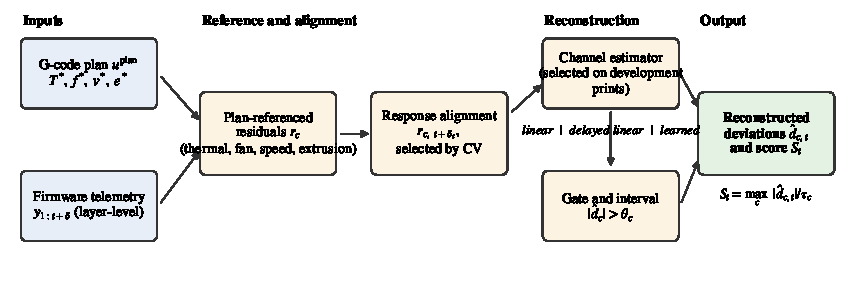
\includegraphics[width=\textwidth]{figs/fig1_architecture.pdf}
\caption{PARD architecture. The G-code plan and firmware telemetry form plan-referenced residuals, which are aligned with the response delay, mapped to deviations by an estimator selected on development prints, gated, and combined into the execution-fidelity score $S_t$.}\label{fig:arch}
\end{figure*}

\subsection{Plan reference and channel observability}
For layer $t$, the residuals are formed from the layer-mean telemetry and the plan values in the original G-code ($T^{*}=\SI{210}{\celsius}$, $f^{*}=1$, $v^{*}=e^{*}=100\%$):
\begin{align}
r_{T,t}&=\bar{T}_t-T^{*}, \qquad r_{C,t}=\bar{f}_t-f^{*},\\
r_{V,t}&=100\left(\frac{\tau^{\mathrm{plan}}_t}{\tau_t}-1\right), \quad r_{E,t}=100\left(\frac{\varepsilon_t}{\varepsilon^{\mathrm{plan}}_t}-1\right),
\end{align}
where $\bar{T}_t$ is the mean hotend temperature, $\bar{f}_t$ the mean reported fan state, $\tau_t$ and $\tau^{\mathrm{plan}}_t$ the observed and planned layer durations, and $\varepsilon_t$ and $\varepsilon^{\mathrm{plan}}_t$ the reported and planned extruded lengths. The planned values are computed from the plan (planned duration $\tau^{\mathrm{plan}}_t$ at nominal speed and planned extruded length $\varepsilon^{\mathrm{plan}}_t$ at nominal flow).

These signals are not all independent physical measurements. The hotend temperature is a measured state. The fan state is a firmware-reported value that closely follows the command, so $r_C$ establishes a reported-command departure, not a measured airflow. The reported extrusion length is the firmware's extrusion value, not a measured material flow rate. The layer-duration ratio is a proxy for the effective execution rate. Throughout, ``deviation'' therefore means a departure of reported execution from the plan.

\subsection{Delay-aware reconstruction}
A heater does not reach a commanded temperature instantly, so the layer in which a temperature step is issued shows only part of it. PARD reads the residual of a later layer:
\begin{equation}
\widehat{d}_{T,t}=f_T\!\left(r_{T,t+\delta_T}\right),
\end{equation}
with $\delta_T\in\{0,1\}$ layers among the candidates and $\delta_T=1$ in the selected configuration (Section~\ref{sec:sel}). The reconstruction therefore carries a latency of about one layer (a median of \layerDur{}~s in these prints). It improves the magnitude estimate and is not an earlier warning.

\subsection{Channel-adaptive estimator selection}\label{sec:sel}
For each channel, three candidate estimators map the reference residual to a deviation. C1 is a linear map of the same-layer residual, $\widehat d_{c,t}=a_c+b_c\,r_{c,t}$. C2 is the same linear map of the next-layer residual, $\widehat d_{c,t}=a_c+b_c\,r_{c,t+1}$. C3 is a gradient-boosted regression-tree model \cite{Friedman2001,Pedregosa2011} on the \nRaw{} telemetry features and the channel residual. Linear maps are fitted by ordinary least squares on the excursion layers of the development prints; the gate in Section~\ref{sec:score} handles nominal layers.

The selection procedure uses only development prints. (i) The mean absolute error of every candidate on excursion layers is computed by five-fold cross-validation grouped by print. (ii) Candidates whose error is at most 10\% above the lowest are eligible. (iii) The simplest eligible candidate is chosen, with the fixed complexity order C1 $<$ C2 $<$ C3. Table~\ref{tab:routing} gives the cross-validated errors and the result. The selected architecture is not arbitrary: delayed linear estimation for temperature, same-layer linear for the fan, and learned estimation for speed and extrusion all follow from the same rule. The candidate set and the rule were refined during development, which is disclosed in Section~\ref{sec:protocol}.

\begin{table}[t]\centering\small
\caption{Development cross-validated MAE on excursion layers (51 development prints, grouped by print); bold marks the selected estimator.}\label{tab:routing}
\adjustbox{max width=\columnwidth}{\input{gen/tab_routing.tex}}
\end{table}

\subsection{Unified execution-fidelity assessment}\label{sec:score}
Each channel estimate passes a gate with threshold $\theta_c$, the 99th percentile of $|\widehat d_{c}|$ over the nominal calibration layers, so that $\tilde d_{c,t}=\widehat d_{c,t}$ if $|\widehat d_{c,t}|>\theta_c$ and zero otherwise. The execution-fidelity score is
\begin{equation}
S_t=\max_{c\in\mathcal{C}}\frac{\left|\tilde d_{c,t}\right|}{\tau_c},
\end{equation}
and a layer is reconstructed as out of tolerance when $S_t>1$. The maximum identifies a departure in any channel instead of averaging it away. The tolerances $\tau_c$ are \tolTh{}~\si{\celsius}, \tolCo{} (fan state), \tolSp{}\% and \tolFl{}\%. They are illustrative engineering thresholds, not certified process specifications, and Section~\ref{sec:robust} varies them. The score does not replace the channel estimates, which are part of the output. For gated excursion layers, a split-conformal interval \cite{Lei2018} $\tilde d_{c,t}\pm q_c$ is reported, with $q_c$ the $(1-\alpha)$ quantile ($\alpha=0.1$) of calibration absolute errors on gated excursion layers. The intervals carry no coverage guarantee under the mixed-excursion shift, and Section~\ref{sec:rel} reports observed coverage.

\section{Experimental methodology}
\subsection{Experimental system and data}
Prints were made on a LulzBot Mini 3 (MET285 tool head) in PLA of \SI{2.85}{mm} diameter. All prints used one calibration-cube G-code, sliced with Cura 4.13.9 for a \SI{0.5}{mm} nozzle at \SI{0.3}{mm} layer height, with 66 layers, a nominal nozzle temperature of \SI{210}{\celsius} and a bed temperature of \SI{60}{\celsius}. Firmware telemetry was aggregated per layer into \nRaw{} features (temperature statistics, heater power, fan state, velocity and extrusion statistics, bed state and layer timing) at a median sampling rate of \samplingHz{}~Hz per layer, with a median layer duration of \layerDur{}~s. [Authors to confirm: logging interface and clock synchronisation.]

The dataset has \layersTotal{} layers from 71 prints. Nine final layers, each of zero duration and a single sample, were excluded, leaving \layersUsed{} layers, of which \layersDev{} are development layers and \layersTest{} are evaluation layers. The prints fall into \nNormal{} nominal prints, \nBed{} bed-adhesion prints with no excursion in the four channels, \nSingle{} single-excursion prints and \nMixed{} mixed-excursion prints (Table~\ref{tab:data}). The 51 development prints are all prints other than the mixed ones. Excursions are deliberate commanded deviations from the plan, introduced as step or gradual schedules. Each mixed print contains one block of \evLenMin{} to \evLenMax{} layers per channel (two for temperature, median block length \evLenMed{} layers), staggered so that blocks overlap.

\begin{table}[t]\centering\small
\caption{Print groups and commanded deviations from plan. Ranges are over excursion layers.}\label{tab:data}
\adjustbox{max width=\columnwidth}{\input{gen/tab_data.tex}}
\end{table}

\subsection{Experimental conditions and evaluation protocol}\label{sec:protocol}
Development and evaluation are separated by print. The development prints are split at random into fitting (70\%) and calibration (30\%) prints; the split was repeated five times (seeds 1--5) and results are reported as the mean and standard deviation over the five splits. Fitting prints train the estimators. Calibration prints set the gate thresholds and conformal quantiles. The \printsTest{} mixed prints are never used for fitting or calibration.

Three stages must be distinguished. In \emph{development}, the candidate estimators, the selection rule, the alignment delay and the initial architecture were created. In \emph{evaluation}, the \printsTest{} mixed prints assess the integrated framework. In \emph{interpretation}, the mixed prints were also examined during refinement, for example when diagnosing the thermal step response and when adding the delayed candidate; the selection rule itself uses development prints only and reproduced the earlier hand-chosen routing. The evaluation therefore has an exploratory component and is not a prospective confirmation of a prespecified framework.

\subsection{Comparison methods and metrics}
Four methods use the same plan information and the same gate and score:
\begin{itemize}
\item B1: same-layer plan residual, $\widehat d_c=r_{c,t}$ without fitting.
\item B2: tuned per-channel residual, a linear map of the same-layer residual (fitted on all fitting layers for temperature and on excursion layers for the other channels).
\item B3: plan-aware learned model, gradient boosting on the \nRaw{} telemetry features, nine plan-geometry features and all four residuals.
\item PARD: the development-selected, delay-aware reconstruction of Section~2.
\end{itemize}
The out-of-tolerance label of a layer is $S^{\mathrm{true}}_t>1$ with $S^{\mathrm{true}}$ computed from the true deviations and the same tolerances; \nOot{} of the \layersTest{} evaluation layers are out of tolerance. The primary metrics are the area under the receiver operating characteristic curve (AUC) of $S_t$ against this label and the F1 score of the decision $S_t>1$, so the decision threshold equals the tolerance and is not tuned. The secondary metrics are the mean absolute error (MAE) of $\widehat d_c$ on excursion layers, the mean score error $|S_t-S^{\mathrm{true}}_t|$, gate recall and false-alarm rate, and interval coverage on gated excursion layers.

\subsection{Statistical analysis and robustness}
The experimental units are prints, which share one geometry, one excursion design and one machine, so the \layersTest{} evaluation layers are not independent. Paired differences between methods use a run-clustered bootstrap (2000 resamples of the \printsTest{} mixed prints, seed-1 split). Robustness is examined by scaling the tolerances by 0.5 and 2 and by an alternative set equal to three standard deviations of each residual on nominal development layers. Coverage is evaluated only on evaluation layers that have a true excursion and pass the gate.

\section{Results}
\subsection{Reconstruction of execution under mixed excursions}
Fig.~\ref{fig:trace} shows PARD output for one evaluation print. The reconstructed deviations follow the commanded blocks in all four channels, and the score $S_t$ exceeds the tolerance during the blocks. Across the evaluation prints, PARD reached an AUC of \aucPard{} ($\pm\,$\aucSdPard{} over five splits) and an F1 score of \fonePard{} ($\pm\,$\foneSdPard{}), against \aucBthree{} and \foneBthree{} for the plan-aware learned model B3, and about \aucBone{} (AUC) and \foneBone{} (F1) for the two residual baselines (Fig.~\ref{fig:comp}a). The mean score error fell from \smaeBthree{} (B3) to \smaePard{}. Against B3 the paired AUC difference was \dAucBthree{} (95\% interval \dAucBthreeLo{} to \dAucBthreeHi{}) and the paired F1 difference was \dFoneBthree{} (\dFoneBthreeLo{} to \dFoneBthreeHi{}); against the tuned residual B2 they were \dAucBtwo{} and \dFoneBtwo{} (Fig.~\ref{fig:comp}b). The intervals describe the observed set of prints and do not include changes of experimental design.

\begin{figure*}[t]\centering
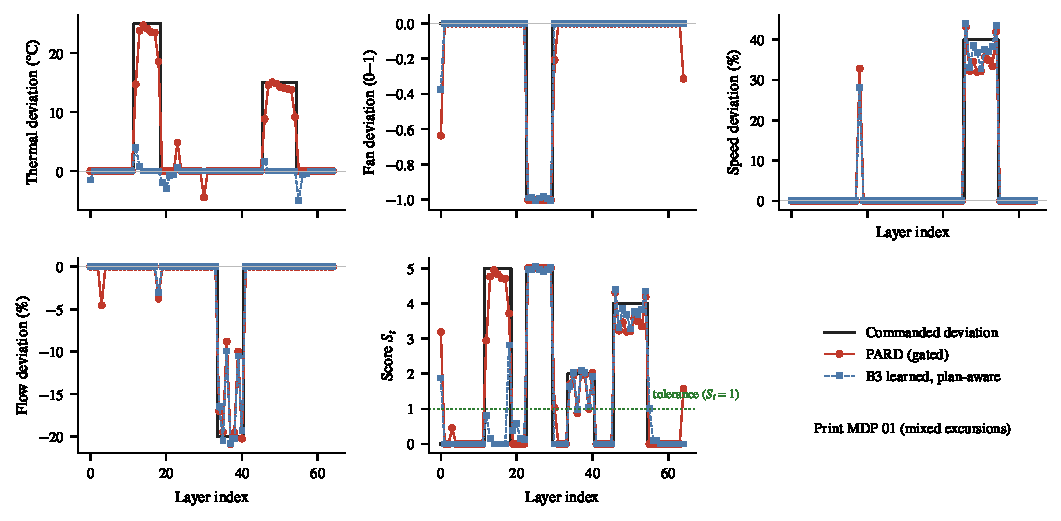
\includegraphics[width=\textwidth]{figs/fig2_trace.pdf}
\caption{Commanded versus reconstructed deviations for one evaluation print (seed-1 split): (a)--(d) the four channels, (e) the execution-fidelity score $S_t$. PARD uses delayed linear estimation for temperature, same-layer linear for fan state and learned estimation for speed and extrusion.}\label{fig:trace}
\end{figure*}

\begin{figure*}[t]\centering
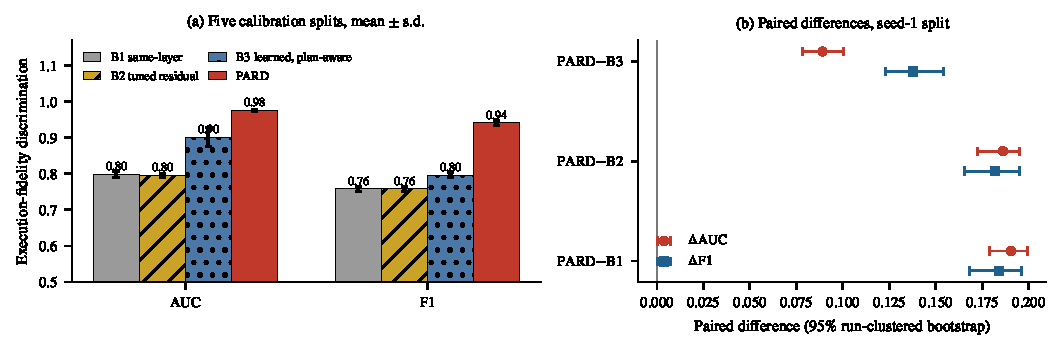
\includegraphics[width=\textwidth]{figs/fig3_comparison.pdf}
\caption{Execution-fidelity discrimination on the \printsTest{} mixed evaluation prints. (a) AUC and F1 of PARD and the three plan-aware baselines (mean $\pm$ s.d.\ over five calibration splits). (b) Paired differences between PARD and each baseline with 95\% run-clustered bootstrap intervals (seed-1 split).}\label{fig:comp}
\end{figure*}

\subsection{Contribution of response alignment and estimator selection}
Thermal alignment explains much of the gap to the learned baseline. With the estimator and fitting rule held fixed, moving from a same-layer residual to a one-layer-delayed residual reduced the temperature-deviation MAE on mixed prints from \thDelayZero{} to \thDelayOne{}~\si{\celsius} (a reduction of \thRedPct\%, Fig.~\ref{fig:delay}a); the tuned same-layer residual B2 gave \maeThBtwo{}~\si{\celsius} (a \thRedBtwoPct\% reduction), and a two-layer delay was worse (\thDelayTwo{}~\si{\celsius}). The learned model B3, which has no delayed input, reached \maeThBthree{}~\si{\celsius}. The development data show the same direction independently of the mixed prints: cross-validated MAE fell from \cvThCone{} to \cvThCtwo{}~\si{\celsius} (\cvThDrop\%). The step response in Fig.~\ref{fig:delay}b gives the reason. In development steps (cold) the measured-to-commanded ratio was \onsetDevZero{} in the onset layer and \onsetDevOne{} one layer later; in the mixed steps (hot) it was \onsetMixZero{}, \onsetMixOne{} and \onsetMixTwo{} in the first three layers, so heating settles more slowly and a one-layer alignment leaves some bias at onset.

\begin{figure*}[t]\centering
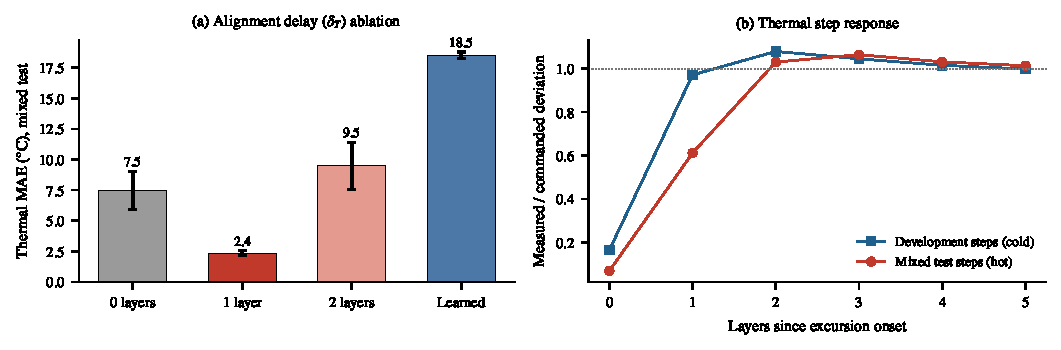
\includegraphics[width=\textwidth]{figs/fig4_delay.pdf}
\caption{Thermal response alignment. (a) Temperature-deviation MAE on mixed evaluation prints for alignment delays of 0, 1 and 2 layers with the same linear estimator, and for the learned model (mean $\pm$ s.d.\ over five splits). (b) Median measured-to-commanded deviation by layers since excursion onset, for development (cold) and mixed (hot) steps with commanded deviation of at least \SI{5}{\celsius}.}\label{fig:delay}
\end{figure*}

The other channels are not improved by delay and are handled by the selection rule. Learned estimation gave MAE of \maeSpPard{}\% for speed and \maeFlPard{}\% for extrusion, against \maeSpBtwo{}\% and \maeFlBtwo{}\% for the tuned same-layer residual. The plan-aware learned model B3 is comparable, with \maeSpBthree{}\% and \maeFlBthree{}\%, which is slightly lower than PARD. For the fan, the same-layer linear estimator was best (\maeCoPard{}). PARD therefore does not outperform every alternative in every channel; its advantage in the unified score comes from combining estimators that suit different channels, chiefly the delayed thermal estimator.

\subsection{Robustness and reliability of the reconstruction}\label{sec:robust}
PARD ranked first on AUC under all four tolerance sets (Table~\ref{tab:sens}), and its F1 score stayed at or above 0.92. Three qualifications apply. The nominal-variability tolerances for speed and extrusion are very wide (\tolBSp\% and \tolBFl\%), so that set mainly tests the thermal and fan channels, and it is reported only as a sensitivity check. The mixed excursions are blocks of \evLenMin{} to \evLenMax{} layers, so whole-block recovery is an easy criterion and is not used as evidence. The one-layer alignment improves magnitude estimates and does not provide earlier detection: with one layer of latency allowed, a same-layer residual also flags the onset.

\begin{table}[t]\centering\small
\caption{Execution-fidelity AUC and F1 under alternative tolerance sets (mean over five splits; bold marks the best method).}\label{tab:sens}
\adjustbox{max width=\columnwidth}{\input{gen/tab_sensitivity.tex}}
\end{table}

\label{sec:rel}Table~\ref{tab:rel} reports reliability for PARD. Gate recall was between \rclSpPard{} and \rclThPard{} and false-alarm rates between \farSpPard{} and \farThPard{} on nominal layers of each channel. Observed interval coverage was \covCoPard{} for the fan but \covThPard{} for temperature, \covSpPard{} for speed and \covFlPard{} for extrusion, below the 0.90 target in three of four channels, and the lowest split value was \covMinThPard{} for temperature. The reported intervals should therefore be read as indicative widths, not calibrated guarantees, under the mixed-excursion shift.

\begin{table}[t]\centering\small
\caption{Reliability of the PARD reconstruction on mixed evaluation prints (mean over five splits). Coverage target 0.90.}\label{tab:rel}
\adjustbox{max width=\columnwidth}{\input{gen/tab_reliability.tex}}
\end{table}

\section{Discussion}
\subsection{Why a common plan reference with channel-adaptive reconstruction}
Direct plan referencing works where the recorded observation is informative, as for temperature once response delay is handled and for the fan state. Learned mapping is preferable where a simple ratio of timing or extruded length is a weak proxy, as for speed and extrusion. In the development prints the selection rule made this assignment without manual intervention, and it matched the assignment found earlier by hand. The contribution is a common reconstruction interface that routes each channel to a suitable estimator, not a universally superior estimator. The thermal result also illustrates why a learned model can fail under changed conditions: all development temperature excursions were cold (\SI{-20}{} to \SI{0}{\celsius}), whereas all mixed excursions were hot (\SI{\thMixMin}{} to \SI{\thMixMax}{\celsius}).

\subsection{Manufacturing relevance}
The reconstruction is suited to execution-record review: comparing reported settings against prescribed conditions, and flagging build intervals whose estimated departure exceeds a stated tolerance for closer inspection. The thermal estimate arrives with about one layer of delay. No reduction in scrap, downtime or part defects is claimed, because none was measured.

\subsection{Generalisation and limitations}
The evidence covers one printer, one material and one geometry. The excursions are scripted, frequent and of similar block length, and the mixed prints share one design, so the paired intervals understate the uncertainty of a broader population. The fan and extrusion channels are firmware-reported values and establish reported-command departures. The tolerances are illustrative and results depend on them. Interval coverage is incomplete, and the evaluation has an exploratory component (Section~\ref{sec:protocol}). A practical next step is evaluation on independently designed excursions, other geometries and machines, and additional physical measurements of flow and cooling.

\section{Conclusions}
This study developed PARD, a plan-referenced framework for reconstructing process-execution deviations in FFF from built-in firmware telemetry. By combining plan references, response-delay alignment and development-selected channel estimators, it provides a unified assessment of reported deviations in temperature, cooling, speed and extrusion. In the evaluated mixed-excursion experiments, PARD reached an execution-fidelity AUC of \aucPard{} and an F1 score of \fonePard{}, ahead of the strongest plan-aware learned baseline by \dAucBthree{} AUC and \dFoneBthree{} F1. One-layer thermal alignment reduced the temperature-deviation error by \thRedPct\% relative to same-layer estimation. The results support combining a common plan reference with channel-dependent reconstruction in the investigated FFF setting. Future work will examine independently designed excursions, broader manufacturing conditions and additional physical measurements.

\section*{Acknowledgements}
[Funding and acknowledgements to be completed by the authors.]

\section*{Data and code availability}
The analysis script that regenerates every number, table and figure in this paper is available from the authors on request. [Authors to confirm repository and licence.]

\begin{thebibliography}{99}\fontsize{8}{9.5}\selectfont
\setlength{\itemsep}{1pt}
\bibitem{Corradini2022} Corradini F, Silvestri M. Design and testing of a digital twin for monitoring and quality assessment of material extrusion process. Addit Manuf 2022;51:102633. https://doi.org/10.1016/j.addma.2022.102633
\bibitem{Werkle2024} Werkle KT, Trage C, Wolf J, M{\"o}hring H-C. Generalizable process monitoring for FFF 3D printing with machine vision. Prod Eng 2024;18:593--601. https://doi.org/10.1007/s11740-023-01234-2
\bibitem{Read2024} Read JR, Seppala JE, Tourlomousis F, Warren JA, Bakker N, Gershenfeld N. Online measurement for parameter discovery in fused filament fabrication. Integr Mater Manuf Innov 2024;13:541--54. https://doi.org/10.1007/s40192-024-00350-w
\bibitem{FuLi2025} Fu T-H, Li D-R. Real-time process monitoring and error correction in material extrusion-based additive manufacturing via multi-output machine learning. J Manuf Process 2025;152:638--56. https://doi.org/10.1016/j.jmapro.2025.08.025
\bibitem{Yu2020} Yu S-Y, Malawade AV, Chhetri SR, Al Faruque MA. Sabotage attack detection for additive manufacturing systems. IEEE Access 2020;8:27218--31. https://doi.org/10.1109/ACCESS.2020.2971947
\bibitem{Moore2017} Moore SB, Gatlin J, Belikovetsky S, Yampolskiy M, King WE, Elovici Y. Power consumption-based detection of sabotage attacks in additive manufacturing. arXiv preprint 1709.01822; 2017.
\bibitem{Ali2025} Ali H, Cano A, Ahmed I. Machine learning-based early detection of malicious G-code manipulations in 3D printing. J Manuf Process 2025;145:211--35. https://doi.org/10.1016/j.jmapro.2025.04.012
\bibitem{Friedman2001} Friedman JH. Greedy function approximation: a gradient boosting machine. Ann Stat 2001;29:1189--232. https://doi.org/10.1214/aos/1013203451
\bibitem{Pedregosa2011} Pedregosa F, Varoquaux G, Gramfort A, et al. Scikit-learn: machine learning in Python. J Mach Learn Res 2011;12:2825--30.
\bibitem{Lei2018} Lei J, G'Sell M, Rinaldo A, Tibshirani RJ, Wasserman L. Distribution-free predictive inference for regression. J Am Stat Assoc 2018;113:1094--111. https://doi.org/10.1080/01621459.2017.1307116
\end{thebibliography}
\end{document}
